\section{Network and data modeling}

\begin{frame}
  \frametitle{Canonical model settings}
  \framesubtitle{Biological microarrays in comparable conditions}

  \begin{overlayarea}{\textwidth}{\textheight}
    \only<1-2>{\begin{colormixin}{100!white}}
    \only<3->{\begin{colormixin}{40!white}}

  \begin{block}{Notations}
    \begin{enumerate}
    \item a set $\mathcal{P} = \{1,\dots,p\}$ of $p$ variables:\\
      these are typically \alert{the genes} (could be proteins);
    \item a sample $\mathcal{N}=\{1,\dots,n\}$ of individuals associated to
      the variables:\\
      these are typically \alert{the microarray} (could be sequence counts).
    \end{enumerate}
  \end{block}

  \vfill

  \begin{block}{Basic statistical model}<2->
    This can be view as
    \begin{itemize}
    \item a \alert{\emph{random  vector} $X$ in $\mathbb{R}^p$}, whose
      $j$th entry is the $j$th variable,
    \item a  \alert{$n$-size sample} $(X^1,  \dots, X^n)$, such
      as $X^i$ is the $i$th microarrays,
      \begin{itemize}
      \item could be independent identically distributed copies (steady-state)
      \item could be dependent in a certain way (time-course data)
      \end{itemize}
    \item  assume  a   parametric  probability  distribution  for  $X$
      (Gaussian).
    \end{itemize}
  \end{block}

  \end{colormixin}

    \only<3->{
      \vspace{-6cm}
        \begin{beamerboxesrounded}[upper=sur:head,lower=sur:bloc,shadow=true]{The data}
          Stacking    $(X^1,\dots,    X^n)$,    we   met    the    usual
          individual/variable table $\mathbf{X}$

        \begin{tikzpicture}
          \node[opacity=.75] at (-3,1.5) {\pgfuseimage{ngs}};
          \node[opacity=.9] at (-2.75,1.25) {\pgfuseimage{ngs}};
          \node[opacity=.95] at (-2.5,1) {\pgfuseimage{microarray}};
          \node at (-2.25,0.75) {\pgfuseimage{microarray}};
          \node[fill=red, text=white,single arrow] 
          (inference) at (0,1) {\sf \scriptsize stacked in}; 
          
          \node at (4.5,1) {%
            $\mathbf{X} = \begin{pmatrix} 
              x_1^1 & x_1^2 & x_1^3 & \dots & x_1^p \\
              \vdots \\
              x_n^1 & x_n^2 & x_1^2 & \dots & x_n^p \\
            \end{pmatrix}$};
        \end{tikzpicture}
      \end{beamerboxesrounded}
    }
  \end{overlayarea}      
  
\end{frame}

\subsection{Statistical dependence}

\begin{frame}
  \frametitle{Modeling relationship between variables (1)}
  \framesubtitle{Independence}
  
  \begin{definition}[Independence of events]
    Two events $A$ and $B$ are independent if and only if
    \begin{equation*}
      \prob(A,B) = \prob(A) \prob(B),
    \end{equation*}
    which is usually denoted by $A \indep B$. Equivalently,
    \begin{itemize}
    \item $A \indep B \Leftrightarrow \prob(A | B) = \prob(A)$,
    \item $A \indep B \Leftrightarrow \prob(A | B) = \prob(A | B^c) $
    \end{itemize}
  \end{definition}

  \begin{example}[class vs party]<2>
    \begin{table}
      \centering
      \begin{tabular}{cc}
        \begin{tabular}{rrr}
        & \multicolumn{2}{c}{party} \\
        class & Labour & Tory \\ \hline
        working & 0.42 & 0.28 \\
        bourgeoisie & 0.06 & 0.24 \\
      \end{tabular} 
      & 
      \begin{tabular}{rrr}
        & \multicolumn{2}{c}{party} \\
        class & Labour & Tory \\ \hline
        working & 0.60 & 0.40 \\
        bourgeoisie & 0.20 & 0.80 \\
      \end{tabular} 
      \end{tabular} 
      \caption{Joint probability (left) vs. conditional probability (right)} 
    \end{table}
  \end{example}
\end{frame}

\begin{frame}
  \frametitle{Modeling relationships between variables (2)}
  \framesubtitle{Conditional independence}
  
  Generalizing  to more  than two  events requires  strong assumptions
  (mutual independence). Better handle with

  \begin{definition}[Conditional independence of events]<2->
    Two events $A$ and $B$ are conditionally independent if and only if
    \begin{equation*}
      \prob(A,B | C) = \prob(A|C) \prob(B|C),
    \end{equation*}
    which is usually denoted by $A \indep B | C$ 
  \end{definition}

  \begin{example}[Does QI depends on weight?]<3->
    Consider  the  events $A  =  "\text{having low  QI}"$,  $B  = \text{"having  low
    weight"}$. \only<3>{Estimating\footnote{stupidly}  $\prob(A,B)$,  $\prob(A)$  and
    $\prob(B)$ in a sample would lead to
    \begin{equation*}
      \prob(A,B) \neq \prob(A) \prob(B)
    \end{equation*}}
  \only<4>{But in fact, introducing $C = \text{"having a given age"}$,
    \begin{equation*}
      \prob(A,B|C) = \prob(A|C) \prob(B|C)
    \end{equation*}}
\end{example}
  
\end{frame}

\begin{frame}
  \frametitle{Limits of correlation for network reconstruction}
  
  \includegraphics<1>[width=.7\textwidth]{cor_plot}

  \includegraphics<2>[width=.7\textwidth]{pcor_plot}
  
\end{frame}

\subsection{Gaussian Graphical models}

\begin{frame}
  \frametitle{Correlation networks}

  \begin{block}{Correlation (association network)}
    Similar expression profile $\rightsquigarrow$ high-correlation
    \begin{enumerate}
    \item Compute the correlation matrix (Pearson, Spearman, \dots)
    \item Predict an edge between two actors if their absolute correlation is above a given threshold
    \end{enumerate}   
  \end{block}
  
  \vfill

  \begin{block}{Questions}
    \begin{itemize}
    \item How to set up the threshold?
    \item If we target actors with similar profiles, why not clustering?
    \item Information is drowned (all actors are correlated \dots)
    \end{itemize}
    
  \end{block}
\end{frame}

\begin{frame}
  \frametitle{Graphical models}
  \begin{block}{Definition}
    A graphical model gives  a graphical (intuitive) representation of
    the dependence structure of a probability distribution, by linking
    
    \begin{enumerate}
    \item a random  vector (or a set of random  variables.)  $X = \{X_1,
      \dots, X_p\}$ with distribution $\prob$, \bigskip
    \item a graph $\mathcal{G} = (\mathcal{P}, \mathcal{E})$ where
      \begin{itemize}
      \item $\mathcal{P}=\{1,\dots,p\}$ is  the set of nodes associated
        to each variable,
      \item $\mathcal{E}$ is a  set of edges describing the dependence
        relationship of $X\sim \prob$.
      \end{itemize}
    \end{enumerate}
   \end{block}

   \vfill

  \begin{block}{Conditional independence graph}<2> It is the \alert{undirected}  graph $\mathcal{G} =
    \{\mathcal{P},    \mathcal{E}\}$ where
    \begin{equation*}
      (i,j) \notin \mathcal{E} \Leftrightarrow X_i \indep X_j | \mathcal{P} \backslash
      \{i,j\}.
    \end{equation*}
  \end{block}

\end{frame}

\begin{frame}
  \frametitle{The Gaussian case}

  \begin{block}{The data}
    \begin{tikzpicture}
      \node[opacity=.75] at (-3,1.5) {\pgfuseimage{microarray}};
      \node[opacity=.9] at (-2.75,1.25) {\pgfuseimage{microarray}};
      \node[opacity=.95] at (-2.5,1) {\pgfuseimage{microarray}};
      \node at (-2.25,0.75) {\pgfuseimage{microarray}};
      \node[fill=red, text=white,single arrow] 
      (inference) at (0,1) {\sf \scriptsize Inference}; 
          
      \node at (4.5,1) {%
        $\mathbf{X} = \begin{pmatrix} 
          x_1^1 & x_1^2 & x_1^3 & \dots & x_1^p \\
          \vdots \\
          x_n^1 & x_n^2 & x_1^2 & \dots & x_n^p \\
        \end{pmatrix}$};
    \end{tikzpicture}
  \end{block}

  \begin{block}{Assuming $f_X(\mathbf{X})$ multivariate Gaussian}
    Greatly simplifies the inference:
    \begin{itemize}
    \item[$\rightsquigarrow$]   naturally   links   independence   and
      conditional   independence  to   the   covariance  and   partial
      covariance,
    \item[$\rightsquigarrow$]  gives a  straightforward interpretation
      to the graphical modeling previously considered.
  \end{itemize}
  \end{block}
\end{frame}


\begin{frame}
  \frametitle{Why Gaussianity helps?}
  \framesubtitle{Case of 2 variables or size-2 random vector}

  Let $X,Y$ be two real random variables.
  
  \begin{definitions}
    \vspace{-.5cm}
    \begin{equation*}
      \cov(X,Y)   =  \E\Big[\big(X-\E(X)\big)\big(Y-\E(Y)\big)\Big]  =
      \E(XY) - \E(X)\E(Y).
    \end{equation*}
    \begin{equation*}
      \rho_{XY} = \cor(X,Y) = \frac{\cov(X,Y)}{\sqrt{\var(X) \ \cdot \ \var(Y)}}.
    \end{equation*}
  \end{definitions}
  
  \begin{proposition}
    \vspace{-.25cm}
    \begin{itemize}
    \item $\cov(X,X) = \var(X) = \E[(X-\E X)(Y-\E Y)]$,
    \item $\cov(X+Y,Z) = \cov(X,Z) + \cov(X,Z)$,
    \item $\var(X+Y) = \var(X) + \var(Y) + \cov(X,Y)$.
    \item $X \indep Y \Rightarrow\cov(X,Y) = 0$.
    \item<2> \alert{$X  \indep Y  \Leftrightarrow \cov(X,Y) =  0$ when
        $X,Y$ are Gaussian}.
    \end{itemize}
  \end{proposition}
\end{frame}

\begin{frame}
  \frametitle{The bivariate Gaussian distribution}

  \begin{columns}
    \begin{column}{.4\textwidth}
      \begin{block}{The Covariance Matrix}
        Let
        \begin{equation*}
          X \sim \mathcal{N}(\mathbf{0}, \boldsymbol\Sigma), 
        \end{equation*}
        with unit variance and $\rho_{XY} = \only<1>{0}\only<2>{0.9}$
        \begin{equation*}
          \boldsymbol\Sigma =
          \begin{pmatrix}
            1 & \only<1>{0}\only<2>{0.9} \\ \only<1>{0}\only<2>{0.9} & 1
          \end{pmatrix}.
        \end{equation*}
        The shape of the 2-D distribution evolves accordingly.
      \end{block}
    \end{column}
    
    \begin{column}{.6\textwidth}
      \includegraphics<1>[height=.8\textheight]{multinorm_nocor}
      \includegraphics<2>[height=.8\textheight]{multinorm_cor}
    \end{column}
  \end{columns}
\end{frame}

\begin{frame}
  \frametitle{Generalization: multivariate Gaussian vector}
  \framesubtitle{Now need partial covariance and partial correlation}
  
  Let $X,Y,Z$ be real random variables.
  \begin{definitions}
    \begin{equation*}
      \cov(X,Y|Z) = \cov(X,Y) - \cov(X,Z)\cov(Y,Z)/\var(Z).
    \end{equation*}
    \begin{equation*}
      \rho_{XY|Z}            =            \frac{\rho_{XY}            -
        \rho_{XZ}\rho_{YZ}}{\sqrt{1-\rho_{XZ}^2}\sqrt{1-\rho_{YZ}^2}}.
    \end{equation*}
  \end{definitions}
  $\rightsquigarrow$  Give   the  interaction  between   $X$  and  $Y$
  \alert{once removed the effect of $Z$}.

  \vfill
  
  \begin{proposition}<2>
    When $X,Y,Z$ are jointly Gaussian, then
    \begin{equation*}
      \alert{\cov(X,Y|Z) = 0  \Leftrightarrow \cor(X,Y|Z) = 0 \Leftrightarrow
      X \indep Y | Z.}
    \end{equation*}
  \end{proposition}
\end{frame}

\begin{frame}
  \frametitle{Important properties of Gaussian vectors}

  \begin{proposition}[Gaussian vector and conditioning]
    Consider a Gaussian vector with the following decomposition
    \begin{equation*}
      Z = \begin{pmatrix}
        Z_1 \\ Z_2
      \end{pmatrix}  \sim   \mathcal{N}(\mathbf{0},\bSigma),   \quad
      \bSigma = \begin{pmatrix}
        \bSigma_{11} & \bSigma_{12} \\
        \bSigma_{21} & \bSigma_{22} \\
      \end{pmatrix},\quad
      \bOmega = \bSigma^{-1} = \begin{pmatrix}
        \bOmega_{11} & \bOmega_{12} \\
        \bOmega_{21} & \bOmega_{22} \\
      \end{pmatrix}.
    \end{equation*}
    Then,
    \begin{equation*}
      Z_2|Z_1=\mathbf{z} \sim
      \mathcal{N}\left(-\bOmega_{22}^{-1}\bOmega_{21}\mathbf{z}, \bOmega_{22}^{-1} \right)
    \end{equation*}
    and
    \begin{equation*}
      \bOmega_{22}^{-1}     =      \bSigma_{22}     -     \bSigma_{21}
      \bSigma_{11}^{-1} \bSigma_{12}.
    \end{equation*}
  \end{proposition}

  \vfill

  \begin{block}{Corollary}
    Partial correlations are related  to the inverse of the covariance
    matrix:
    \begin{equation*}
      \cor(Z_i,Z_j|Z_k, k\neq i,j) = - \frac{\Omega_{ij}}{\sqrt{\Omega_{ii}\Omega_{jj}}}
  \end{equation*}
  \end{block}

\end{frame}

\begin{frame}
  \frametitle{Gaussian Graphical Model: canonical settings}

  \begin{block}{Biological experiments in comparable Gaussian conditions}
    Profiles  of  a set  $\mathcal{P}  =  \{1,\dots,p\}$  of genes  is
    described by $X\in\mathbb{R}^p$ such as
    \begin{enumerate}
    \item  $X\sim\mathcal{N}(\boldsymbol\mu,\boldsymbol\Sigma)$,  with
      $\boldsymbol\Theta = \bSigma^{-1}$ the precision matrix.
    \item a sample $(X^1, \dots, X^n)$ of exp. stacked in an $n\times
      p$ data matrix $\mathbf{X}$.
    \end{enumerate}
  \end{block}

  \begin{overlayarea}{\textwidth}{\textheight}
        
        \begin{block}{Conditional independence structure}
          \vspace{-.5cm}
          \begin{equation*}
            (i,j)  \notin  \mathcal{E}  \Leftrightarrow  X_i  \indep  X_j  |
            X_{\backslash \{i,j\}} \Leftrightarrow \Theta_{ij} = 0.
          \end{equation*}
        \end{block}
        
        \vspace{-.5cm}
        \begin{block}{Graphical interpretation}
          \vspace{-.5cm}
          \begin{center}
            \begin{tabular}{c@{\hspace{2cm}}c}
              \begin{tabular}{c}
                \small $\mathcal{G}=(\mathcal{P},\mathcal{E})$ \\
                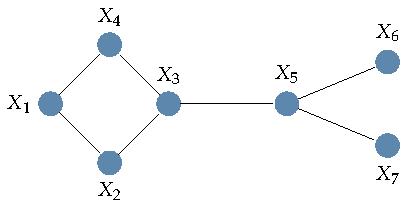
\includegraphics[width=.3\textwidth]{graph}
              \end{tabular}
              &
              \begin{tabular}{c}
                \small $\bTheta$\\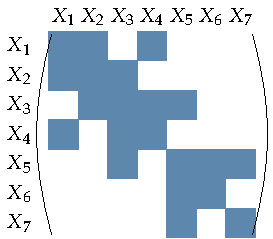
\includegraphics[width=.2\textwidth]{Markovadjacency}
              \end{tabular}
            \end{tabular}
          \end{center}
        \end{block}
        \vspace{-1cm}
        $\rightsquigarrow$ \alert{``Covariance'' selection}
   
  \end{overlayarea}      
\end{frame}

\begin{frame}
  \frametitle{Gaussian Graphical Model and Linear Regression}

  \begin{block}{Linear regression viewpoint}
    Gene expression $X_i$ is linearly explained by the other genes':
    \begin{equation*}
      X_i | X_{ \setminus i} = - \sum_{j \neq i}
      \frac{\Theta_{ij}}{\Theta_{ii}} X_j + \varepsilon_i,\quad \varepsilon_i
      \sim \mathcal{N}(0,\Omega_{ii}^{-1}), \quad \varepsilon_i \perp X
      \end{equation*}
      Conditional  on its  neighborhood,  other profiles  do not  give
      additional insights
    \begin{equation*}
      X_i | X_{ \setminus i} = \sum_{\alert{j \in \text{neighbors}(i)}} \beta_j X_j + \varepsilon_i
      \quad         \text{with         }         \beta_j         =
      -\frac{\Theta_{ij}}{\Theta_{ii}}.
    \end{equation*}
  \end{block}

  \alert{$\rightsquigarrow$ ``Neighborhood'' selection}

\end{frame}


\begin{frame}
  \frametitle{Gaussian Graphical Model and AR process (1)}
  
  \begin{block}{Time course data}
    Time course- data experiment can  be  represented  as   a  multivariate  vector
    $X=(X_1,\dots,X_p)\in\mathbb{R}^p$,  generated  through a
    \alert{first order vector autoregressive} process $VAR(1)$:
    \begin{equation*}
      X^{t}   =   \boldsymbol\Theta   X^{t-1}   +   \mathbf{b}   +
      \boldsymbol\varepsilon^{t},\quad t \in [1,n]
    \end{equation*}
    where  $\boldsymbol\varepsilon^{t}$ is  a white  noise to  ensure  the Markov
    property and $X^{0} \sim \mathcal{N}(0, \boldsymbol\Sigma^0)$.
  \end{block}

   \vfill
 
   \begin{block}{Consequence: a Gaussian Graphical Model}<2>
     \begin{itemize}
     \item        Each       $X^{t}        |        X^{t-1}       \sim
       \mathcal{N}(\mathbf{\theta}X^{t-1}, \boldsymbol\Sigma)$, 
     \item  or,  equivalently,  $X_j^{t}  |  X^{t-1}  \sim
       \mathcal{N}(\boldsymbol\Theta_jX^{t-1}, \boldsymbol\Sigma)$
     \end{itemize}
     where $\boldsymbol\Sigma$ is known and $\boldsymbol\Theta_j$ is the
     $j$th row of $\boldsymbol\Theta$.
   \end{block}
 \end{frame}

\begin{frame}
  \frametitle{Gaussian Graphical Model and AR process (2)}
  \framesubtitle{Interpretation as a GGM}

  \begin{block}{The VAR(1) as a covariance selection model}
    \begin{equation*}
      \theta_{ij} = \frac{\mathrm{cov}\left(X^t_i,X^{t-1}_j|
          X^{t-1}_{\mathcal{P}\backslash j} \right)} 
      {\mathrm{var}\left(      X^{t-1}_j|X^{t-1}_{\mathcal{P}\backslash
            j}\right)},
    \end{equation*}
  \end{block}

  \vfill
  
    \begin{block}{Graphical Interpretation}
      $\rightsquigarrow$                   The                  matrix
      $\boldsymbol\Theta=(\theta_{ij})_{i,j\in\mathcal{P}}$  encodes the
      network $\mathcal{G}$ we are looking for.
    
      \begin{scriptsize}
        \begin{tikzpicture}
          %% LES DONNÉES
          \node     at     (5,0)     {\begin{tabular}{@{}c@{}}     \sf
              \alert{conditional} dependency between
              $X^{t-1}_{j}$ and $X^{t}_i $\\
              or\\
              non-null partial correlation between $X^{t-1}_{j}$ and $X^{t}_i $\\
              $\Updownarrow$ \\
              $\theta_{ij} \neq 0$\\
            \end{tabular}
          };
        
          \node[fill=red,double  arrow,text=white]  at  (0,0) {if  and
            only if};
        
          %% UN GRAPH
          \tikzstyle{every                  state}=[fill=gray!60!white,
          draw=none,text=black,scale=0.75, transform shape]
          \tikzstyle{every edge}=[->,>=stealth',shorten >=1pt,auto,thin,draw]
          
          % troisième cluster
          \node[state] (C1)  at (-2,0.25) {$i$};  \node[state] (C2) at
          (-3,-0.25) {$j$};
        
          \path (C2) edge [bend left] node [above right] {?}  (C1);
        
        \end{tikzpicture}
      \end{scriptsize}
    \end{block}

\end{frame}

\begin{frame}[fragile]
  \frametitle{Gaussian Graphical Model and AR process (3)}
  \framesubtitle{Graphical interpretation}
  
    \begin{enumerate}
    \item Follow-up of one single experiment/individual; 
    \item Close enough time-points to ensure 
      \begin{itemize}
      \item \alert<1>{dependency} between consecutive measurements;
      \item \alert<2>{homogeneity} of the Markov process.
      \end{itemize}
    \end{enumerate}

  % \vfill
  
  \begin{overlayarea}{\textheight}{\textwidth}
    \only<1>{
   %   \begin{center}
      \begin{tikzpicture}
        \tikzstyle{every state}=[fill=orange!80!white,
        draw=none,text=black,scale=0.7]
        \tikzstyle{every edge}=[->,>=stealth',shorten >=1pt,auto,thin,draw]
        
        \node (x1) [state] at (0,0) {$X_1$};
        \node (x2) [state] at (1,-1) {$X_2$};
        \node (x3) [state] at (-1,-1) {$X_3$};
        \node (x4) [state] at (0,1.5) {$X_4$};
        \node (x5) [state] at (2.5,-1) {$X_5$};
        \path[->,=< stealth] 
        (x1) edge[bend right] (x2)
        (x1) edge (x3)
        (x1) edge (x4)
        (x2) edge (x5)
        (x2) edge[bend right] (x1);
       
          \node at (4,0) {stands for}; 
      %    \node at (4,0) {stands for};
        % First line:
        \node (x_11) [state] at (6,2) {$\mathbf{X}^{t}_1$}; 
        \node (x_12) [state] at (8,2) {$\mathbf{X}^{t+1}_1$}; 
        % Second line: 
        \node (x_21) [state] at (6,1) {$\mathbf{X}^{t}_2$}; 
        \node (x_22) [state] at (8,1) {$\mathbf{X}^{t+1}_2$}; 
       % Third line: 
       \node (x_32) [state] at (8,0) {$\mathbf{X}^{t+1}_3$}; 
       % Fourth line:
       \node (x_42) [state] at (8,-1) {$\mathbf{X}^{t+1}_4$}; 
       \node (x_g1) at (6.5,-1) {\LARGE $\mathcal{G}$};    
        % Fifth line:
       \node (x_52) [state] at (8,-2) {$\mathbf{X}^{t+1}_5$};        
        \path[->] 
        (x_11) edge (x_22)
        (x_11) edge (x_32)
        (x_11) edge (x_42)
        (x_21) edge (x_52)
        (x_21) edge (x_12);
      \end{tikzpicture}
 %     \end{center}
    }
    \only<2>{
      \centering
      \begin{tikzpicture}
        \tikzstyle{every state}=[fill=orange!80!white,
        draw=none,text=black,scale=0.7]
        \tikzstyle{every edge}=[->,>=stealth',shorten >=1pt,auto,thin,draw]
        % First line:
        \node (x_11) [state] at (-5,2) {$\mathbf{X}^{t}_1$}; 
        \node (x_12) [state] at (-2,2) {$\mathbf{X}^2_1$}; 
        \node (x_13) [state] at (1,2) {$\dots$};
        \node (x_14) [state] at (4,2) {$\mathbf{X}^{n}_1$};
        % Second line: 
        \node (x_21) [state] at (-5,1) {$\mathbf{X}^{1}_2$}; 
        \node (x_22) [state] at (-2,1) {$\mathbf{X}^{2}_2$}; 
        \node (x_23) [state] at (1,1) {$\dots$}; 
        \node (x_24) [state] at (4,1) {$\mathbf{X}^{n}_2$}; 
        % Third line: 
        \node (x_31) [state] at (-5,0) {$\mathbf{X}^{1}_3$};
        \node (x_32) [state] at (-2,0) {$\mathbf{X}^{2}_3$}; 
        \node (x_33) [state] at (1,0) {$\dots$}; 
        \node (x_34) [state] at (4,0) {$\mathbf{X}^{n}_3$}; 
        % Fourth line:
        \node (x_41) [state] at (-5,-1) {$\mathbf{X}^{1}_4$};
        \node (x_42) [state] at (-2,-1) {$\mathbf{X}^{2}_4$}; 
        \node (x_43) [state] at (1,-1) {$\dots$}; 
        \node (x_44) [state] at (4,-1) {$\mathbf{X}^{n}_4$};
        \node (x_g1) at (-3.5,-1.5) {\LARGE $\mathcal{G}$};
        \node (x_g2) at (-.5,-1.5) {\LARGE $\mathcal{G}$}; 
        \node (x_g3) at (2.5,-1.5) {\LARGE $\mathcal{G}$};
        
        % Fifth line:
        \node (x_51) [state] at (-5,-2) {$\mathbf{X}^{1}_5$};
        \node (x_52) [state] at (-2,-2) {$\mathbf{X}^{2}_5$}; 
        \node (x_53) [state] at (1,-2) {$\dots$};
        \node (x_54) [state] at (4,-2) {$\mathbf{X}^{n}_5$};
        
        \path[->] 
        (x_11) edge (x_22)
        (x_11) edge (x_32)
        (x_11) edge (x_42)
        (x_21) edge (x_52)
        (x_21) edge (x_12);
        
        \path[->]
        (x_12) edge (x_23)
        (x_12) edge (x_33)
        (x_12) edge (x_43)
        (x_22) edge (x_53)
        (x_22) edge (x_13)

        (x_13) edge (x_24)
        (x_13) edge (x_34)
        (x_13) edge (x_44)
        (x_23) edge (x_54)
        (x_23) edge (x_14);
      \end{tikzpicture}
    }

  \end{overlayarea}
  
\end{frame}

